% bei Standalone in documentclass noch:
% \RequirePackage{luatex85}

\documentclass[captions=tableheading, titlepage= firstiscover, parskip = half , bibliography=totoc]{scrartcl}
%paper = a5 für andere optinen
% titlepage= firstiscover
% bibliography=totoc für bibdateien
% parskip=half  Veränderung um Absätze zu verbessern

\usepackage{scrhack} % nach \documentclass
\usepackage[aux]{rerunfilecheck}
\usepackage{polyglossia}
\usepackage[style=numeric, backend=biber]{biblatex} % mit [style = alphabetic oder numeric] nach polyglossia
\addbibresource{lit.bib}
\setmainlanguage{german}

\usepackage[autostyle]{csquotes}
\usepackage{amsmath} % unverzichtbare Mathe-Befehle
\usepackage{amssymb} % viele Mathe-Symbole
\usepackage{mathtools} % Erweiterungen für amsmath
\usepackage{fontspec} % nach amssymb
% muss ins document: \usefonttheme{professionalfonts} % für Beamer Präsentationen
\usepackage{longtable}

\usepackage[
math-style=ISO,    % \
bold-style=ISO,    % |
sans-style=italic, % | ISO-Standard folgen
nabla=upright,     % |
partial=upright,   % /
]{unicode-math} % "Does exactly what it says on the tin."
\setmathfont{Latin Modern Math}
% \setmathfont{Tex Gyre Pagella Math} % alternativ

\usepackage[
% die folgenden 3 nur einschalten bei documenten
locale=DE,
separate-uncertainty=true, % Immer Fehler mit ±
per-mode=symbol-or-fraction, % m/s im Text, sonst \frac
]{siunitx}

% alternativ:
% per-mode=reciprocal, % m s^{-1}
% output-decimal-marker=., % . statt , für Dezimalzahlen

\usepackage[
version=4,
math-greek=default,
text-greek=default,
]{mhchem}

\usepackage[section, below]{placeins}
\usepackage{caption} % Captions schöner machen
\usepackage{graphicx}
\usepackage{grffile}
\usepackage{subcaption}

% \usepackage{showframe} Wenn man die Ramen sehen will

\usepackage{float}
\floatplacement{figure}{htbp}
\floatplacement{table}{htbp}

\usepackage{mhchem} %chemische Symbole Beispiel: \ce{^{227}_{90}Th+}


\usepackage{booktabs}

 \usepackage{microtype}
 \usepackage{xfrac}

 \usepackage{expl3}
 \usepackage{xparse}

 % \ExplSyntaxOn
 % \NewDocumentComman \I {}  %Befehl\I definieren, keine Argumente
 % {
 %    \symup{i}              %Ergebnis von \I
 % }
 % \ExplSyntaxOff

 \usepackage{pdflscape}
 \usepackage{mleftright}

 % Mit dem mathtools-Befehl \DeclarePairedDelimiter können Befehle erzeugen werden,
 % die Symbole um Ausdrücke setzen.
 % \DeclarePairedDelimiter{\abs}{\lvert}{\rvert}
 % \DeclarePairedDelimiter{\norm}{\lVert}{\rVert}
 % in Mathe:
 %\abs{x} \abs*{\frac{1}{x}}
 %\norm{\symbf{y}}

 % Für Physik IV und Quantenmechanik
 \DeclarePairedDelimiter{\bra}{\langle}{\rvert}
 \DeclarePairedDelimiter{\ket}{\lvert}{\rangle}
 % <name> <#arguments> <left> <right> <body>
 \DeclarePairedDelimiterX{\braket}[2]{\langle}{\rangle}{
 #1 \delimsize| #2
 }

\setlength{\delimitershortfall}{-1sp}

 \usepackage{tikz}
 \usepackage{tikz-feynman}

 \usepackage{csvsimple}
 % Tabellen mit \csvautobooktabular{"file"}
 % muss in table umgebung gesetzt werden


% \multicolumn{#Spalten}{Ausrichtung}{Inhalt}

\usepackage{hyperref}
\usepackage{bookmark}
\usepackage[shortcuts]{extdash} %nach hyperref, bookmark

\newcommand{\ua}[1]{_\symup{#1}}
\newcommand{\su}[1]{\symup{#1}}


\title{Versuch 353}
\subtitle{Das Relaxationsverhalten eines RC-Kreises}
\author{Sebastian Pape\\
        sepa@gmx.de \and
        Jonah Nitschke\\
        lejonah@web.de}
\date{Durchführung: 24.01.2017\\
      Abgabe: 31.01.2017}

\begin{document}
\maketitle
\setcounter{page}{1}

\section{Theorie}

In dem Versuch V353 wurde das Relaxationsverhalten eines $RC$-Kreises untersucht.
Relaxation bedeutet, dass ein System aus seinen Ruhezustand gebracht wird
und nicht-oszillatiorisch in diesen zurückkehrt.
Mit einem $RC$-Kreis ist solch ein Relaxationsverhalten zu erreichen. Mit verschiedenen
Messmethoden soll die $RC$-Konstante bestimmt werden, sodass diese miteinander
verglichen werden können. Darüberhinaus soll die Eigenschaft des $RC$-Kreises als
Integrator nachgewiesen werden.

\subsection{Ent- und Aufladevorgang}

Bei dem Entladevorgang eines Kondensators mit der Kapazität $C$ über einen Widerstand
$R$ lässt sich die Ladung auf dem Kondensator als Funktion der Zeit darstellen.
Es ergibt sich unter der Randbedingung $Q(\infty) = 0$ die folgende Formel.

\begin{equation}
  \label{eqn:Entladen}
  Q(t) = Q(0)\cdot \exp{(-\frac{t}{RC})}
\end{equation}

Für den Aufladevorgang gelten die Randbedingungen $Q(0) = 0$ und $Q(\infty) = CU_0$. Dabei ist $U_0$ die Spannung der Spannungsquelle. Damit ergibt sich
die folgende Formel des Aufladevorgangs eines Kondensators über einen Widerstand.

\begin{equation}
  \label{eqn:aufladen}
  Q(t) = CU_0(1 - \exp{(-\frac{t}{RC})})
\end{equation}

$RC$ wird auch \emph{spezifische Zeitkonstante} genannt, da dieser Ausdruck ein Maß
der Geschwindigkeit des Entladevorgangs darstellt.
Nach $\tau = RC$ ändert sich die Ladung des Kondensators um den Faktor $0,368$. Nach $2,3\tau$ sind nur noch 10\% des Ausgangswertes der Ladung auf dem
Kondensator vorhanden.

\subsection{Relaxationsverhalten bei periodischer Anregung}

Wird nun an den $RC$-Kreis eine periodische Spannung $U(t) = U_0\cos{\omega t}$
anstelle einer einzelnen Erregung angelegt ändert sich das Relaxationsverhalten
mit der Frequenz $\omega$. Ist $\omega \ll \frac{1}{RC}$ sind die
Spannungen des Generators und des Kondensators näherungsweise in Phase.
Je hochfrequenter die Spannung wird, desto deutlicher wird die Phase
zwischen den beiden Spannungen.
Für $\omega\rightarrow\infty$ nähert sich die Phasenverschiebung asymptotisch
den Wert $\frac{\pi}{2}$.

\subsection{Der RC-Kreis als Integrator}

Mit Hilfe eines $RC$-Kreises lässt sich die angeschlossene Spannung $U(t)$
unter der Voraussetzun $\omega\gg\frac{1}{RC}$ integireren. Dies hängt damit zusammen, dass die Kondensatorspannung $U_C(t)$
proportional mit dem Integral von $U(t)$ zusammenhängt.
Unter der gestellten Bedingung gilt näherungsweise der Zusammenhang

\begin{equation}
  \label{eqn:Integrator}
  U_C(t) = \frac{1}{RC}\int_0^tU(t')\symup{d}t'.
\end{equation}

Daran ist erkenntlich, dass sich die Kondensatorspannung $U_C(t)$ als Integrator
der Generatorspannung $U(t)$ eignet.

\section{Durchführung}

Zu Beginn des Versuches wird der $RC$-Kreis aufgebaut. Eine Schaltplanskizze
ist in Abb. \ref{fig:Aufbau} zu sehen.
Mit dieser Schaltung kann der Auf- und Entladevorgangs des Kondensators
über das Oszilloskop beobachtet werden. Dazu wird der Generator auf den
Rechteckspannungsbetrieb eingestellt und das Oszilloskop so geregelt, dass
die Lage des Spannungsnullpunktes zu sehen ist. Während des Suchvorganges des
Spannungsnullpunktes wird die Periodendauer der Rechteckspannung möglichst groß gewählt.
Sobald eine geeignete Kurve gefunden wurde, kann diese
als Bild gespeichert werden.

Danach wird der Generator auf den Sinusspannunsbetrieb umgestellt, sodass
der $RC$-Kreis bei variirender Frequenz untersucht werden konnte.
Die Amplitude der Kondensatorspannung wird bei insgesamt 15 verschiedenen
Frequenzen beobachtet. Dabei werden fünf Frequenzen aus dem nieder
frequenten Bereich zwischen $10$ bis $\SI{100}{\hertz}$ betrachtet. Die
anderen zehn Frequenzen werden aus dem Frequenzbereich zwischen $200$ bis
$\SI{1100}{\hertz}$ in hunderter Schritten gewählt. Bei der Messung wird
neben der Frequenz und Kondensatorspannung auch die Generatorspannungen betrachtet.

Desweiteren wird der Phasenunterschied zwischen Generator- und Kondensatorspannung
in Abhängigkeit von der Frequenz gemessen. Dafür werden die beiden Spannungen
auf die Eingänge des Oszilloskops gelegt. Es werden der Abstand der beiden
Nulldurchgänge, sowie die Periodendauer der Generatorspannung mit Hilfe
des digitalen Periodendauermessgerät, welches in dem Oszilloskop integriert ist
gemessen.

Abschließend wird die Eigenschaft der Kondensatorspannung als Integrator
der Generatorspannung untersucht. Dafür wird die Frequenz maximal geregelt,
sodass sie der Bedingung $\omega$ >> $\frac{1}{RC}$ genügt. Bei dem verwendeten
Generator ist die Minimalfrequenz bei ca. $\SI{4}{\hertz}$ erreicht.
Nun wird die Generatorspannung parallel zu der Kondensatorspannung auf dem
Oszilloskop ausgegeben und bei geeigneten Einstellungen als Bild gespeichert.
Die Messung wird mit einer Sinusspannung, einer Rechteckspannung und einer
Dreieckspannung durchgeführt.\\

\FloatBarrier
\begin{figure}
  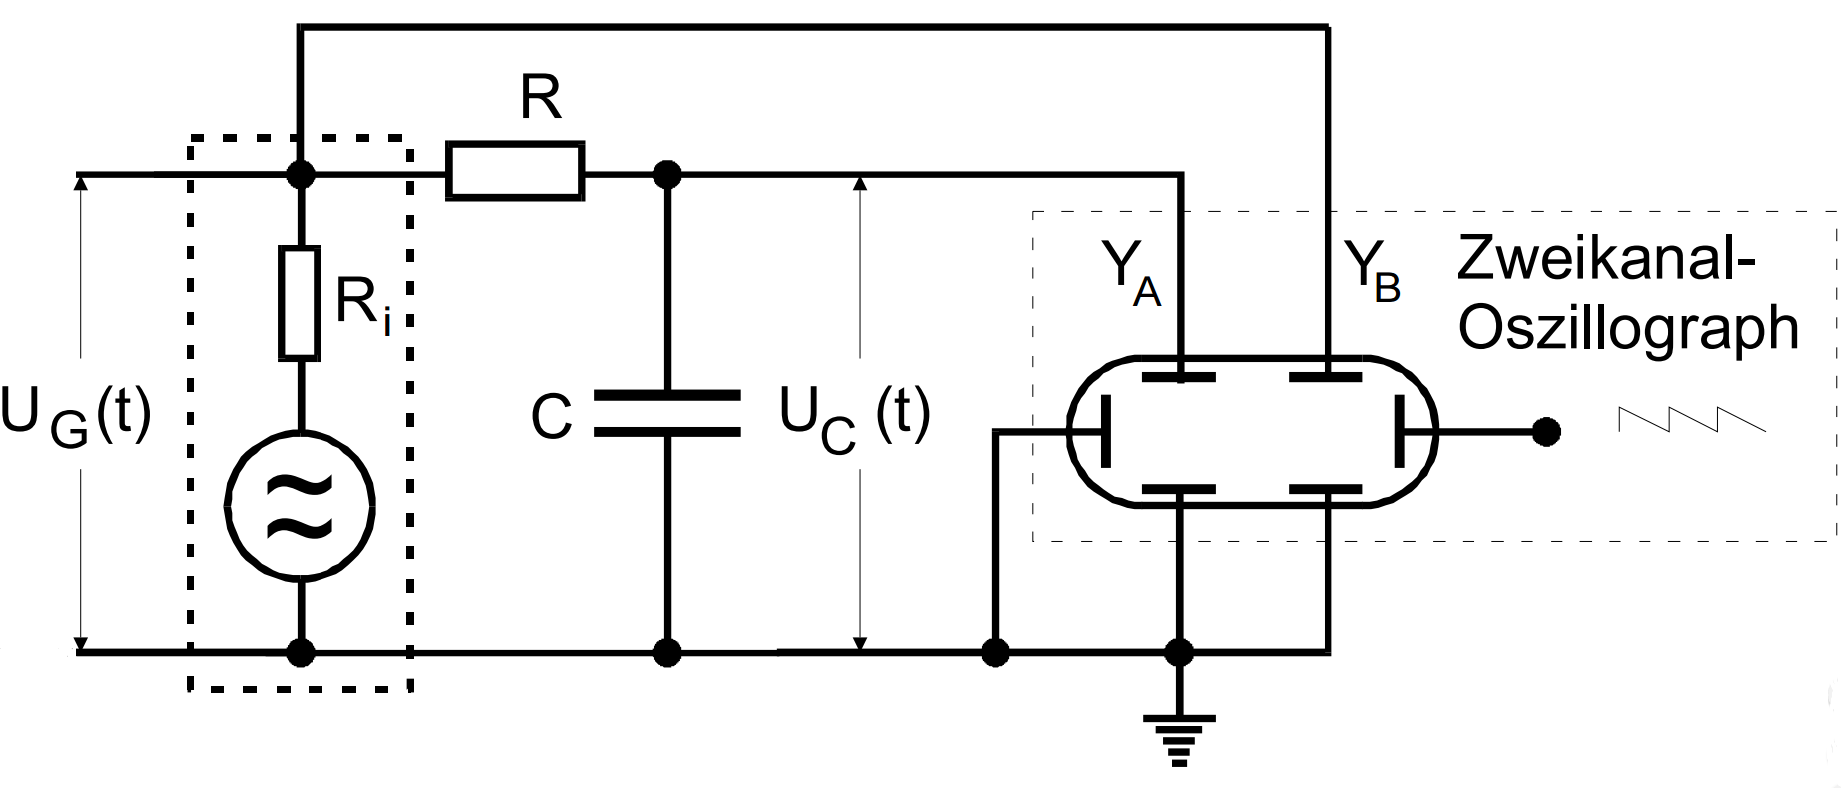
\includegraphics[width=\textwidth]{Aufbau_V353.PNG}
  \caption{Schaltplanskizze des verwendeten RC-Kreises}
  \label{fig:Aufbau}
\end{figure}

Der in Abbildung \ref{fig:Aufbau} dargestelle Schaltplan zeigt den verwendeten
RC-Kreis. Die Spannung $U\ua{G}$ beschreibt die Generatorspannung. Der Widerstand
R steht für den Innenwiderstand des Generators. Der verwendete Widerstand ist mit
dem Buchstaben R und der Kondensator mit C gekennzeichnet. Die Spannung $U\ua{C}$
symbolisiert die Kondensatorspannung. Die Eingänge des Oszillographen sind mit
$Y\ua{A}$ und $Y\ua{B}$ dargestellt. Die Generatorspannung wird auf den
$Y\ua{B}$-Eingang des Oszillographen gelegt und die Kondensatorspannung auf den
$Y\ua{A}$-Eingang.

\newpage

\section{Auswertung}

Bei den folgenden Rechnungen werden die Fehler mit der Gaußschen Fehlerfortpflanzung
berechnet, wobei hierfür die automatische Fehlerrechnung mittels des Ufloat-Paketes
von Python genutzt wird.
Bei den Rechnungen werden die folgenden Konstanten für die Normalbedingungen, die
Umgebungstemperatur und die Länge des Gasbehälters ($\su{b}$), sowie die Übersetzung ($\su{\ddot{U}}$)
verwendet:

\begin{align*}
  \su{T}\ua{0} &= \SI{273.15}{K} \\
  \su{p}\ua{0} &= \SI{1.0132}{bar} \\
  \su{T}       &= \SI{293.15}{K} \\
  \su{b}       &= \SI{0.05}{m} \\
  \su{\ddot{U}}       &= 5.046
\end{align*}

\subsection{Bestimmung der Wellenlänge}

Die Wellenlängen ergeben sich dabei aus den gemessenen Werten mit der Formel \eqref{eqn:lambda},
wobei die gemessenen Werte als fehlerfrei angenommen werden. Die berechneten Werte
sind in der folgenden Tabelle eingetragen:

\begin{table}
  \centering
  \caption{Gemessene Intensitätsmaxima ($\su{z}$) und die daraus resultierende Wellenlänge.}
  \label{tab:Wellenlängen}
  \begin{tabular}{c c c}
    \toprule
    $\increment d$ in $\si{mm}$ & $\su{z}$ & $\lambda$ in $\si{nm}$ \\
    \midrule
    0.355 & 1051 & 675.05 \\
    0.339 & 1002 & 676.41 \\
    0.351 & 1044 & 671.98 \\
    0.349 & 1036 & 673.34 \\
    0.343 & 1013 & 676.89 \\
    0.343 & 1031 & 665.07 \\
    0.345 & 1027 & 671.52 \\
    0.347 & 1034 & 670.81 \\
    0.347 & 1029 & 674.07 \\
    0.343 & 1022 & 670.93 \\
    \bottomrule
  \end{tabular}
\end{table}

Durch das Mitteln der bestimmten Wellenlängen (Tabelle \ref{tab:Wellenlängen})
ergibt sich für die Wellenlänge des verwendeten Lasers ein Wert von $\lambda \,
= \, (672.6 \pm 1.1) \, \si{nm}$, wobei es sich bei dem Fehler um die
Standardabweichung handelt.

\subsection{Bestimmung des Brechungsindexes von Luft und Kohlenstoffdioxid}

Mit den anfangs angegebenen Werten und den Formeln \eqref{eqn:n_Druck} und \eqref{eqn:delta_n} lässt sich aus der
gemessenen Anzahl an Intensitätsmaxima ($\su{z}$) und der Druckdifferenz ($\increment
\su{p}$) der Brechungsindex von Luft sowie von Kohlenstoffdioxid bestimmen. Bei
$\increment \su{n}$ handelt es sich hier nicht um den Fehler sondern die Differenz des
Brechungsindexes, der Fehler wird durch $\sigma\ua{n}$ angegeben.

\begin{table}
  \centering
  \caption{Gemessene Intensitätsmaxima ($\su{z}$) und der daraus resultierende Brechungsindex für Luft.}
  \label{tab:IndexLuft}
  \begin{tabular}{c c c c c}
    \toprule
    $\increment \su{p}$ in $\si{bar}$ & $\su{z}$ & $\increment \su{n}$ & $\su{n}$ & $\sigma\ua{n} * 10^{6}$ \\
    \midrule
    0.76 & 35 & 0.000235 & 1.000337 & 0.543 \\
    0.8  & 34 & 0.000229 & 1.000311 & 0.501 \\
    0.8  & 34 & 0.000229 & 1.000311 & 0.501 \\
    0.8  & 35 & 0.000235 & 1.000320 & 0.516 \\
    0.82 & 35 & 0.000235 & 1.000312 & 0.503 \\
    0.83 & 35 & 0.000235 & 1.000308 & 0.497 \\
    0.8  & 34 & 0.000229 & 1.000311 & 0.501 \\
    0.81 & 35 & 0.000235 & 1.000316 & 0.509 \\
    0.82 & 35 & 0.000235 & 1.000312 & 0.503 \\
    0.8  & 33 & 0.000222 & 1.000302 & 0.486 \\
    \bottomrule
  \end{tabular}
\end{table}

Die Fehler ergeben sich mittels Gauß´scher Fehlerfortpflanzung durch folgende
Formel:

\begin{align}
  \label{eqn:FehlerDelN}
  \sigma\ua{\increment n} &= \frac{1}{2} \frac{\su{z}}{\su{b}} \cdot \sigma\ua{\lambda} \\
  \label{eqn:FehlerN}
  \sigma\ua{n}            &= \frac{\su{T}}{\su{T}\ua{0}} \frac{\su{p}\ua{0}}{\increment \su{p}} \cdot \sigma\ua{\increment n}
\end{align}

Mit den Werten aus Tabelle \ref{tab:IndexLuft} ergibt sich für den Brechungsindex
von Luft folgender Wert:

\begin{equation*}
  \su{n}\ua{Luft} = (1.000314 \pm 0.000001)
\end{equation*}

Äquivalent dazu lässt sich auch der Brechungsindex von Kohlenstoffdioxid berechnen.
Die gemessenen Werte sowie der jeweilige Brechungsindex sind in folgender Tabelle
eingetragen:

\begin{table}
  \centering
  \caption{Gemessene Intensitätsmaxima ($\su{z}$) und der daraus resultierende Brechungsindex für Kohlenstoffdioxid.}
  \label{tab:IndexLuft}
  \begin{tabular}{c c c c c}
    \toprule
    $\increment \su{p}$ in $\si{bar}$ & $\su{z}$ & $\increment \su{n}$ & $\su{n}$ & $\sigma\ua{n} * 10^{6}$ \\
    \midrule
    0.8  & 58 & 0.000390 & 1.000530 & 0.855 \\
    0.8  & 50 & 0.000336 & 1.000457 & 0.737 \\
    0.64 & 36 & 0.000242 & 1.000411 & 0.663 \\
    0.6  & 39 & 0.000262 & 1.000475 & 0.766 \\
    0.56 & 37 & 0.000249 & 1.000483 & 0.779 \\
    0.52 & 35 & 0.000235 & 1.000492 & 0.794 \\
    0.48 & 29 & 0.000195 & 1.000442 & 0.712 \\
    0.44 & 28 & 0.000188 & 1.000465 & 0.750 \\
    0.4  & 25 & 0.000168 & 1.000457 & 0.737 \\
    0.37 & 24 & 0.000161 & 1.000474 & 0.765 \\
    \bottomrule
  \end{tabular}
\end{table}

Die Fehler werden dabei wieder nach Formel \eqref{eqn:FehlerDelN} und \eqref{eqn:FehlerN}
berechnet. Für den Brechungsindex von Kohlenstoffdioxid ergibt sich damit der
folgende Wert:

\begin{equation*}
  \su{n}_{\ce{CO_2}} = (1.000469 \pm 0.000001)
\end{equation*}

\section{Diskussion}

Bei Vergleich der gemessenen Werte mit den Literaturwerten (Tabelle \ref{tab:Vergleich})
wird erkenntlich, dass die bestimmten Größen in der richtigen Größenordnung liegen
und auch nicht zu stark von den Literaturwerten abweichen. Jedoch liegt keiner
dieser Werte im Fehlerintervall des experimentell bestimmten Wertes.

\begin{table}
  \centering
  \caption{Vergleich der experimentell bestimmten Werte mit den Litearturwerten.}
  \label{tab:Vergleich}
  \begin{tabular}{c c c}
    \toprule
    & Experimenteller Wert  & Literaturwert \\
    \midrule
    $\lambda$ in in $\si{nm}$ & 672.6 \pm 1.1         & 632.8         \\
    $\su{n}\ua{Luft}$              & 1.000314 \pm 0.000001 & 1.000292      \\
    $\su{n}_{\ce{CO_2}}$          & 1.000469 \pm 0.000001 & 1.000449      \\
    \bottomrule
  \end{tabular}
\end{table}

Die auftretenden
Abweichungen lassen sich auf mehrer Ursachen zurückführen. Einerseits war die
verwendete Messdiode so empfindlich, dass schon bei kleinen Erschütterungen am
Messaufbau Interferenzmaxima registriert wurden. Ein weitere Fehlerquelle kann
auch das Ablesen der Wegstrecke der Spiegelverschiebung an der Mikrometerschraube
sein, da die nur in gewissem Maße genau ist.

Vor allem bei der Bestimmung des Brechungsindexes von Kohlenstoffdioxid ist die
Gaskammer eine Fehlerquelle. Es befand sich immer ein kleiner Restanteil an Luft
in der Kammer, so dass die gemessenen Werte nicht für reines Kohlenstoffdioxid
gelten. Um diesen Fehler so gering wie möglich zu halten, wurden jedoch mehrere
Messungen gemacht.

Da die bestimmten Werte jedoch alle den Literaturwerten ähneln, sind die auftretenden
Fehler vermutlich ausschließlich statistischer Natur.


\end{document}
